%!TEX root = main.tex
\chapter{État de l'art}
\chaptertable

%\section{La visualisation et manipulation 3D collaborative sur web}

\section{Modélisation 3D collaborative}

\subsection{Collaboration et concurrence dans un Environnement Virtuel 3D}
Dans un contexte collaboratif, on considère qu'il n'est pas possible pour une 
personne seule de réaliser la tâche proposée complètement. 
La modélisation 3D collaborative permet à différents concepteurs de travailler 
ensemble sur une même tâche de manière efficace (en terme de coût temporel et 
financier) et avec un support visuel manipulable, éditable et flexible (proposant 
différentes possibilités de visualisation). 
En se complétant, leur travail peut aussi entrer en conflit, se compenser, 
s'annuler\ldots
La mise en place de solutions pour ces situations dépend de nombreux facteurs 
comme le type de collaboration (synchrone, asynchrone) et de cohérence souhaité 
(forte, éventuelle) par exemple.

Les différentes solutions pour la conception collaborative peuvent être divisés en 
trois types: 
\begin{enumerate*}[label=(\roman*)]
	\item les mécanismes de type autoritaires (requérant des autorisations),
	\item les opérations de transformation et 
	\item les autres solutions synchrones et asynchrones.
\end{enumerate*}
Selon leurs comportements face à l'apparition d'un conflit, ces types de 
collaboration sont classifiés comme pessimistes ou optimistes (Tableau 
\ref{table:collprobs}). Les solutions de type autoritaire (\og \textit{authoritative}\fg{}) 
sont comptés parmi les solutions pessimistes car elles préviennent toute 
occurrence de conflit tandis que les solutions des deux autres types,
transformées opérationnelles -- \gls{OT} -- et autres (synchrone ou asynchrone), 
sont dites optimistes car permissives face à l'apparition de conflits. 
Dans ce dernier cas, les conflits détectés peuvent, selon les stratégies, amener à 
une résolution manuelle ou automatique.

\begin{table}
	\centering
	\caption{Solutions conventionnelles pour les problèmes collaboratifs 
	\cite{Yu2016}.}
	
	\small
	\label{table:collprobs}
	\begin{tabular}{ m{0.20\textwidth}  m{0.35\textwidth} m{0.35\textwidth}}\hline
		\textbf{Type}& \textbf{Mécanismes de Collaboration} & \textbf{Problème 
		résolu}    \\ \hline
		\multirow{4}{*}{Autoritaire}                     & Verrou                        & 
		\multirow{4}{*}{Évitement des conflits}                                          \\
		& Feux de circulation  
		&                                                                                  \\
		& Droits d'accès               
		&                                                                                  \\
		& Permission temporaire        
		&                                                                                  \\ \hline
		\multirow{2}{0.2\textwidth}{Transformées opérationnelles}                     & 
		Séquence de transformation                     & Résolution de conflit temps-réel 
		pour les documents textuels                     \\ \cline{2-3} 
		& Transformées opérationnelles 3D                 & Résolution de conflit pour 
		dépendant des modèles 3D                              \\ \hline
		\multirow{3}{0.2\textwidth}{Autre (synchrone ou asynchrone)} & 
		Semi-synchrone                               & \multirow{3}{0.3\textwidth}{Détection 
		de conflit ou résolution avec interaction utilisateur} \\
		& Signalisation des conflit %(conflict awareness) 
		&                                                                                  \\
		& Résolution de conflit créative                 &                      \\ 
		\bottomrule                                                           
	\end{tabular}
\end{table}


La plupart du temps ce sont des mécanismes autoritaires comme le mécanisme 
de verrouillage (\textit{lock mechanism}), des feux de signalement (\textit{traffic 
light mecanism}) ou requérant des droits ou des permissions temporaires, qui sont 
proposés dans les solutions collaboratives traditionnelles. Les utilisateurs doivent 
souscrire aux permissions du système avant de pouvoir effectuer leurs 
modifications. Ces mécanismes permettent de s'assurer que les opérations sont 
effectuées de manière séquentielle ce qui assure la cohérence des données à 
travers le système. Plus simples à mettre en place, ces mécanismes sont plus 
restrictifs vis à vis de la liberté de création des utilisateurs du système. Par 
exemple, Lets3D \cite{Ha2015} est un éditeur collaboratif 3D sur le web dont la 
gestion de la concurrence repose sur la demande de permission par objet 
sélectionné (ce qui verrouille l'objet pour les autres utilisateurs lorsqu'elle est 
accordée).

 Avec ceux d'Ellis et Gibbs, les travaux de Greenberg et Marwood sont parmi les 
premiers à s'intéresser aux problèmes liés à la gestion de la concurrence dans 
un système distribué au sein d'un collecticiel \cite{Ellis1989,Greenberg1994}. 
Alors que Duplex \cite{Pacull1994}, un \gls{EVC3D}, est présenté au même 
moment, se dernier s'intéresse plus spécifiquement aux problématiques de 
passage à l'échelle en essayant de réduire la taille du contexte partagé pour 
limiter les problèmes liés à la concurrence. 
Les modèles liés à l'annulation (\textit{undo/redo}) dans les éditeurs collaboratifs 
distribués sont nombreux. Pour les documents textuels, les travaux les plus 
aboutis dans un environnements distribué collaboratif 
\cite{Prakash1994,Sun2002,Ressel}. Les 
algorithmes souvent utilisés dans ce cadre sont les algorithmes 
de  transformées opérationnelles -- \gls{OT} -- \cite{Ellis1989} ou les algorithmes 
de réplication de  données commutatives -- \glspl{CRDT} -- \cite{Shapiro2007} 
s'orientant de plus en plus vers des solutions décentralisées pour un usage à 
grande échelle \cite{Weiss2009a}.
\subsection{... sur le web : HTML5 et au delà}
%TODO designing in context
%\cite{Dobos2015}

L'arrivée du web a bouleversé les usages liés à la collaboration sur des objets 3D. 
Les principes, les technologies, l'omniprésence du web en ont fait une plateforme 
de prédilection pour la visualisation et la manipulation d'objet 3D de haut niveau.   
Pour les projets d'\gls{AIC} ou de \gls{BIM}, la demande de traitement et la fidélité 
ont tendance à être plus élevés, particulièrement pour la représentation de dessins 
d'ingénierie ou de modèles d'architecture 3D. 
Les objets simples (primitives) ou les maillages optimisés pour le rendu temps-réel 
ne sont ni suffisants ni assez génériques pour être supportés par tous les 
processus liés à l'élaboration d'un produit. 
Plus les projets sont gros, plus ils dépendent d'une multitude de logiciels 3D --  
dont l'interopérabilité n'est pas garantie -- s'adressant chacun aux besoins d'une 
tâche spécifique. 
Chaque tâche (ex: modélisation \gls{CAO}, \textit{stress testing}\ldots) possède sa 
propre représentation des données qui peut varier selon les niveaux de 
sémantique attachés à la géométrie. 
Pour garder une trace de ces données et mettre en commun les données 
générées autour d'un produit, l'utilisation d'un \gls{PDM}/\gls{PLM} est 
souvent requise. Bien que certains outils de création d'objets 3D (par exemple 
Autodesk Revit) autorisent la synchronisation de fichier via leur dépôt à distance, 
ce n'est généralement pas applicable aux générations suivantes. 
En cela, une plateforme web pour un \gls{PDM}/\gls{PLM} à 
l'avantage d'être distribuée pour être accessible depuis un navigateur web ; avec 
un système d'édition hors-ligne, le téléversement peut s'avérer long et fastidieux.
De plus, les logiciels spécialisés pour la modélisation 3D, contrairement aux jeux 
multijoueurs, sont traditionnellement dédiés à un utilisateur unique sans 
représentation visuelle des autres opérateurs dans le même espace 3D. 
Ici encore, les principes d'accessibilité du web facilitent la création d'un espace 
virtuel 3D collaboratif pour la visualisation, la manipulation et l'échange de
données partagées. 


La collaboration en temps-réel est de plus en plus présente sur le web pour 
différents types de documents notamment 3D.
La revue sur la visualisation distribuée, effectuée par Grimstead et al. en 2005 
\cite{Grimstead2005}, indique que la plupart des systèmes sont conçus pour 
moins de cent 
utilisateurs simultanés et reposent sur un ou plusieurs serveurs pour supporter ces 
utilisateurs. 
Ils expliquent ce schéma par la volonté du fournisseur de service d'assurer une 
qualité de service et la sécurité du système. 
Les systèmes de \gls{RV} collaboratifs font exception à ce schéma où l'utilisation 
des réseaux \gls{P2P} est plus répandue pour supporter parfois plus d'un millier 
d'utilisateurs simultanés. 
Dans chacun des cas, chaque système a besoin d'un client adapté pour opérer de 
manière isolée sans inter-opérer avec les autre systèmes. 
C'est dans ce contexte qu'en 2011, Mouton et al. \cite{Mouton2011} présentent 
une analyse approfondie de l'état des environnements collaboratifs 3D, ciblant 
principalement la visualisation collaborative. 
Ils montrent l'apparition de la tendance à déporter les environnements collaboratifs 
sur le web grâce à l'évolution d'XMLHttpRequest en client-serveur et l'apparition du 
standard HTML5 comprenant un support avancé de l'audio et de la vidéo ainsi que 
plusieurs \gls{API} de stockage côté client (LocalStorage, IndexedDB). 
Les applications web revêtent plusieurs avantages par rapport aux applications 
natives sur mobiles ou aux logiciels autonomes. 
Cela repose principalement sur le fait que les navigateurs sont présents partout 
dans nos vies aujourd'hui (2017), incluant les téléphones intelligents et les 
tablettes qui les rendent indépendants des plateformes utilisées. 
Le déploiement sur le web ne requiert pas d'installation ou de mises à jour autre 
que celle du navigateur (en ne considérant que les applications sans greffon). 
La modification de l'application est gérée de manière centralisée par les serveurs 
qui distribuent l'application. 
Les éditeurs peuvent diffuser leur application à l'échelle mondiale instantanément  
et la mettre à disposition des utilisateurs sans dépendre d'un réseau de distribution 
autre qu'internet.

%Computer-Aided Engineering (CAE) Collaborative /


Parmi les solutions sans greffon (\textit{plugin less}), beaucoup sont développées 
pour faire de la modélisation 3D  et utilisent l'architecture client-serveur et le 
protocole 
\gls{WebSocket} pour effectuer la synchronisation entre les différents les clients 
collaborateurs. Quelques raisons peuvent expliquer cette situation :
\begin{enumerate}
	\item développement : connaissance du standard \gls{WebSocket} par les 
	développeurs (historique)
	\item gestion des données : simplification de la synchronisation des données 
	(centralisé)
	\item suivi de l'utilisateur : dépendance de l'utilisateur vis à vis de la connexion 
	au serveur et donc du service (engagement) 
\end{enumerate}

Parmi les solutions commerciales comme OnShape, Clara.io et TinkerCAD le 
choix de plateformes web dans l'infonuagique pour la modélisation \gls{CAO} est 
prépondérant souvent assorti d'un gestionnaire de version et d'une plateforme de 
diffusion des création.
OnShape est un service de modélisation 3D très riche dont l'objectif est de 
proposer une qualité équivalente des fonctionnalités de modeleurs autonomes 
(\textit{standalone}) professionnels, le tout de manière collaborative. Leur approche 
de la gestion de version développe le concept de micro version \cite{Baran2015}. 
Cette approche est employée dans les travaux de Lu et al. \cite{Lu2016} pour gérer 
l'évolution de productions participatives liées à des tâches de modélisation 3D 
en usant de la créativité, de l'intelligence et du savoir-faire 
d'un grand nombre de personnes en sous-traitance (\textit{crowdsourcing}). Le 
modeleur 3D Clara.io \cite{Houston2013} est plus généraliste. Il s'oriente 
davantage vers des fonctionnalités avancées de rendu 3D sur le \textit{cloud} en 
utilisant du lancer de rayons. 
Les fonctionnalités d'historisation et de collaboration proposées 
dans Clara.io restent très basiques (seulement annuler~/~refaire). TinkerCAD 
est aussi une plateforme de publication d'objets 3D pour faciliter l'accès à la 
conception d'objets 3D. TinkerCAD est une application destinée au grand 
public pour la conception et l'impression 3D. De ce fait, les fonctionnalités sont 
limitée à cause du métier, l'impression 3D et de la cible, grand public. La gestion 
de version est donc plus légère, similaire à celle proposée par Clara.io. 
OpenJSCAD, Verold Studio, Vectary sont d'autres 
exemples de modeleurs 3D moins connus avec des fonctionnalités proches de 
TinkerCAD.
Un peu à part, GrabCAD est une plateforme web plus orientée sur la gestion de 
données 3D \gls{CAO} (\gls{PLM}) qui possède un système de gestion de version 
performant et une système d'annotation et de visualisation collaborative.
Pour réduire l'empreinte mémoire des messages transmis lors de la collaboration 
sur le web, certains systèmes d'édition collaborative de contenu 3D utilisent une 
modélisation par surface implicite (BlobTree) \cite{Grasberger2013}. 
Les objets sont alors manipulés comme des géométries de construction de 
solides avec les opérations booléennes associées. 
Le Tableau \ref{table:encoding} résume les différents types 
d'encodage associé au type de modélisation 3D. 
\improve{tableau comparatif gestion historique ou versionning}
\improve{tableau comparatif de GrabCAD, OnShape, clara.io}
%
%\begin{table}[]
%	\centering
%	\caption{Comparaison de fonctionnalités entres modeleurs 3D basés web}
%	\label{my-label}
%	\begin{tabular}{@{}cccc@{}}
%		&  Client serveur & P2P &  Collaboratif\\ \midrule
%		Claro.io        & c        & g       & o       \\
%		GrabCAD                  & c        & g       & o       \\
%		OnShape &          &         &         \\
%		&          &         &         \\ \bottomrule
%	\end{tabular}
%\end{table}


\subsection{Web 3D : deux approches}
La plateforme web possède certains avantages par rapport à des clients lourds. 
En effet, le développement de l'infonuagique a permis le développement de 
meilleures infrastructures de services. Du fait de ce développement, la création de 
plateformes collaboratives sur le web pour faire de la conception 3D est devenue 
non seulement faisable en termes de ressources mais également en termes de 
technologie. Il existe deux types d'approches pour créer du contenu web 2D ou 
3D. L'approche déclarative et l'approche impérative. La Figure \ref{fig:impdec} 
montre le pendant 3D pour chaque approche 2D. En 2D, les spécifications 
déclaratives (\gls{SVG}) et impératives (canvas) sont issues du \gls{HTML}5 alors 
qu'en 3D, les spécifications sont encore en évolution. 

\begin{figure}[hbt]
	\centering
	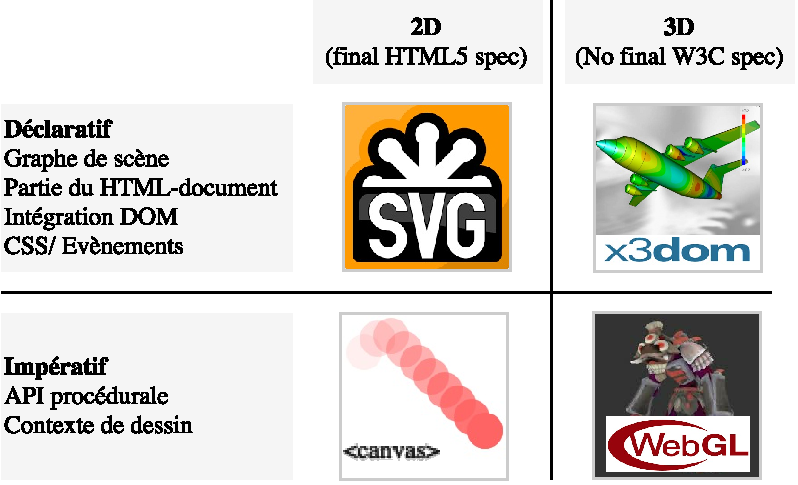
\includegraphics[width=0.7\columnwidth]{impdec}
	\caption{Déclaratif vs Impératif en 2D et en 3D sur le web}
	\label{fig:impdec}
\end{figure}

L'approche déclarative (Dec3D) s'intègre au \gls{DOM} et se 
focalise sur l'utilisation les technologies du web existantes comme CSS3, 
HTML5 et l'Ajax. 
X3D est ainsi un format de fichier respectant le standard ISO \cite{X3D2011} pour 
représenter des scènes 3D interactives en XML, rétro-compatible avec VRML97. Il 
se différencie des formats de fichier type Collada en intégrant le comportement de 
la scène durant l'exécution en plus de la description du contenu 3D. Les deux 
bibliothèques les plus notables dérivées de ce standard sont X3DOM 
\cite{Behr2010} et XML3D \cite{Sons2010} : toutes les deux sont capables de 
supporter les récentes avancées de WebGL pour afficher une scène décrite dans 
le \gls{DOM} à l'intérieur d'un \textit{canvas} HTML5. 
X3DOM essaye de respecter le standard X3D et ses concepts pour en permettre 
l'intégration du format dans le \gls{DOM}. De plus, X3DOM intègre le support 
d'élément \gls{HTML}, les évènements \gls{DOM} et de profils \acrshort{CSS} en 
supplément \cite{Sutter2015}. 
En comparaison avec X3DOM, XML3D a développé une extension à \gls{HTML}5 
pour décrire une scène 3D. 
L'utilisation d'un langage déclaratif basé sur XML comme X3D est bien 
adapté pour le contenu 3D utilise des données CAO/MAO ou WCS dans des 
applications \gls{SIG} car il peut être directement transformé (ex. XSLT) d'une 
représentation à une autre (tout comme le X3D peut être rendu dans un navigateur 
en utilisant X3DOM). 

L'approche déclarative est utilisée dans de nombreux travaux de visualisation 
scientifique 3D distribuée \cite{Jung2012} pour des données spatiales 
\cite{Stein2014} ou du rendu volumique \cite{Becher2012} par exemple. 
En manipulant directement les objets 3D à partir des éléments \gls{DOM}, grâce à 
sa structure bien connue, il est alors plus simple lors de la collaboration d'utiliser 
ces éléments \cite{Gadea2016} ou les évènements du \gls{DOM} \cite{Lowet2009} 
comme protocole de synchronisation de scènes. 
L'ajout de nombreux \textit{listeners} sur un document peut affecter les 
performances de parcours de l'arbre du \gls{DOM} notamment si une scène est
très peuplée.
%declarative XML- based languages such as X3D are suited well for SOAs in that 
%3D content, such as CAD/ CAM data or a given WCS response in a GIS 
%application, can be directly transformed, e.g. via an XSLT or similar transform, 
%from one representa- tion to another (such as an X3D world that can be rendered 
%in 
%real-time in the web browser using the X3DOM frame- work).

%TODO BIM CAD PLM 
%TODO Building Information Modeling: The Web3D Application for AEC 
%\cite{Campbell2007}
%TODO WEB3D, COLLABORATIVE DESIGN AND PLM Enrico Vezzetti (1), 
%Maria Grazia Violante (2)
%\info{webrtc collaborative visual analysis \cite{Li2015} }
%\info{webrtc medical \cite{Andrikos2015}}
%\info{webrtc x3dom \cite{Stein2014} \cite{Andrioti2015} }
%\info{webrtc webgl \cite{Desprat2015} \cite{Desprat2016} SAGE2 
%\cite{Marrinan2008} }

\begin{figure}[hbt]
	\centering
	\includegraphics[width=0.9\columnwidth]{webglstats.eps}
	\caption{Support de WebGL 1 (2014-2017) et WebGL 2 
		(2016-2017)}
	\label{fig:webglstats}
\end{figure}

Concernant l'approche impérative, la spécification WebGL 1.0 \cite{Khronos2011} 
proposée par le groupe Khronos permet aux navigateurs d'effectuer un rendu 3D 
grâce à une \gls{API} JavaScript adaptée de l'\gls{API} d'OpenGL~ES~2.0 
\cite{Khronos2007} en utilisant l'élément \textit{canvas} d'\gls{HTML}5. Cette 
spécification est supportée par la plupart des navigateurs traditionnels (Chrome 
depuis v49, Firefox depuis v52, Safari depuis v9.1, IE 11\footnote{Le contexte 
	WebGL est accessible depuis <<~\texttt{experimental-webgl}~>> au lieu de 
	<<~\texttt{webgl}~>>.\label{fn:webglcontext}}, Edge 14\textsuperscript{ 
	\ref{fn:webglcontext}} et Opera depuis v41) ainsi que les navigateurs mobiles 
	(iOS 
Safari depuis v9.3, Android Browser depuis v53 et Chrome for Android depuis v53) 
à l'exception d'Opera Mini\footnote{Données issues de 
	\url{http://caniuse.com/\#search=webgl}, consulté le 26/11/2016.}. La 
	spécification 
WebGL 2.0 \cite{Khronos2016} basée sur OpenGL~ES~3.0 \cite{Khronos2008}, 
déjà publiée en tant que brouillon, est en phase 
expérimentale\footnote{\url{http://caniuse.com/\#feat=webgl2} consulté le 
	26/11/2016}.\improve{add some example of coviz web} La Figure 
\ref{fig:webglstats} montre l'évolution du support de WebGL~1 et WebGL~2 durant 
ces dernières années sur les différentes plateformes possédant un navigateur 
web\footnote{Images capturées sur \url{https://webglstats.com/}. Les statistiques 
	sont collectées à partir de sites partenaires de \url{webglstats.com}. Ces sites 
	sont en 
	ciblent des néophytes de la WebGL possédant donc le matériel 
	dédié à la 3D en général. Consulté le 04/07/2017.}.



\begin{table}[h]
	\centering
	\caption{Encodage des données transmises}
	\label{table:encoding}
	\begin{tabular}{@{}lcc@{}}\hline
		\textbf{Référence}& \textbf{Modélisation 3D}   & 
		\begin{tabular}[c]{@{}l@{}}\textbf{Encodage des}\\ 
			\textbf{modifications}\end{tabular} \\ \midrule
		\cite{Grasberger2013}        &      Blob (CSG)    & Fonction implicite        \\
		Clara.io \cite{Houston2013}               & Polygonale       &  Commande 
		interface     \\
		\cite{Mouton2014}                  & Polygonale       & Fonction paramétrique     \\
		OnShape \cite{Baran2015} &    Paramétrique      &     Microversion    \\
		cSculpt \cite{Calabrese2016} &      Polygonale    &    Fréquence spatiale  \\ 
		\bottomrule
	\end{tabular}
\end{table}

\section{Communication en temps-réel}
L'expression temps-réel est largement utilisé par des applications requérant une 
forme de temps de réponse rapide et réactif pour que l'utilisateur ait une bonne 
expérience. La communication dans un \gls{EVC} particulièrement pour permettre aux utilisateurs de s'immerger dans la collaboration et faire confiance à l'application (exactitude des modifications).


La communication et la transmission des données lors de la collaboration un des 
aspects prépondérant dans les \gls{EVC3D} concerne . Que ce soit dans dans un 
\gls{EV}, un jeu multi-joueur ou un jeu sérieux (\textit{serious game}), les 
participants interagissent en temps-réel ou quasi-réel alors qu'ils sont situés à 
différents endroits géographiques. 
Le développement d'un \gls{EVC3D} nécessite donc des connaissances issues de 
plusieurs domaines comme la conception et l'implémentation de protocoles 
réseaux et de réseaux distribués.

Un protocole de communication en temps-réel existe, il s'appelle \gls{RTP} et a 
été développé dans le but de faciliter la communication en temps-réel sur un 
réseau. Coexistant avec \gls{RTP}, le protocole \gls{RTCP} est utilisé pour 
transmettre des informations de contrôle à propos des données en temps-réelles. 
\gls{RTCP} transporte des données contenant des informations de contrôle et des 
informations statistiques concernant les flux de données et les connexions des 
destinataires qui permettent à l'expéditeur d'ajuster le flux en conséquence. Les 
protocoles \gls{RTP} et \gls{RTCP} sont principalement conçus pour la 
transmission de flux audio et vidéo, moins pour des données arbitraires comme 
des données 3D. Pour cette raison, leur utilisation est limitée dans le cadre des 
\gls{EVC} pour la modélisation 3D. 

Du fait de la variété des domaines et applications auxquels s'adressent les 
\glspl{EVC3D} existants, il n'existe pas de protocole de 
communication parfait adapté à tous les types d'environnement. 
Les besoins en communication qui se formulent souvent en termes de 
fiabilité de la livraison des messages et de l'ordonnancement des messages sont 
les variables d'ajustement en fonction des contraintes qu'imposent les limites de 
temps de réponse et de bande passante.

\subsection{Fiable versus Non Fiable}

La fiabilité d'un protocole de communication définit comment le protocole fait face 
à la perte ou au retard de données. Un protocole dit \og fiable\fg{} (\textit{reliable}) 
fait en sorte de rendre sûr le fait que le destinataire recevra éventuellement les 
données envoyées par l'expéditeur. Lors de la perte d'un paquet, ou lorsqu'il est 
retenu quelque part dans le réseau, le protocole est au courant et essaye de 
renvoyer les données concernées. Un protocole dit \og non fiable\fg{}, ne fournit 
pas ce genre de garantie et n'essaiera pas de transmettre à nouveau les données.

Bien que la fiabilité dans une communication est une propriété habituellement 
recherchée, cela implique également que le canal doit connaître l'état des données 
qui transitent. Soit l'expéditeur numérote les paquets en séquence, et dans ce 
cas, seul le destinataire à la connaissance des paquets manquants (et à 
renvoyer). Pour indiquer les paquets manquants à l'expéditeur, le destinataire peut 
envoyer des acquittements (ACKs) pour confirmer leur réception. Ces ACKs 
peuvent être joints aux messages ou envoyés séparément. En plus des données 
additionnelles envoyées, un protocole fiable peut aussi générer des latences 
sévères (dans l'attente d'un paquet perdu ou avec beaucoup de retard). Cela peut 
impliquer que les \og nouvelles\fg{} données peuvent arrivées et être déjà 
périmées.

Pour certaines applications qui ne peuvent pas faire face à ces délais potentiels 
ou ne peuvent pas s'offrir de données additionnelles, les protocoles non fiables 
sont utilisés. 
L'expéditeur se repose alors sur le réseau pour délivrer les paquets 
correctement, mais il n'y a aucune garantie. Les protocoles non fiables ne 
nécessitent pas de données additionnelles (séquence de nombre ou ACKs). 
L'expéditeur n'est cependant jamais sûr que le destinataire a reçu toutes ses 
données. Lorsque le destinataire a une connaissance du type de trafic qu'il reçoit, 
il peut fournir un retour à l'expéditeur pour qu'il ajuste le flux de paquets. Ce 
principe est appliqué par le protocole \gls{RTCP}, conjointement avec \gls{RTP}, 
pour fournir les données statistiques liés à la  connexion à l'expéditeur.

L'utilisation d'un protocole de communication fiable ou non fiable dépendant du 
type d'application et du type de l'environnement réseau dans lequel il est conçu 
pour opérer. Si une application dite temps-réel est conçue pour fonction en réseau 
local -- \gls{LAN} -- l'utilisation d'un protocole fiable est une option recommandée. 
Les câbles utilisés dans ce contexte sont souvent rapides et stables ; un packets 
perdu ou corrompu peut rapidement être détecté et retransmis. Dans des 
environnements réseaux sont moins prévisibles comme les \gls{MAN} ou 
\gls{WAN}, la nature de l'application a une influence importante sur le type de 
protocole à utiliser. Selon si la pertinence des données est de courte durée, ou si 
la perte de données n'est pas aussi importante que le fait de la retarder, alors un 
protocole non fiable peut être employé.


\subsection{Ordonné versus Désordonné}
Les paquets envoyés par l'expéditeur ne prennent pas forcément tous le même 
chemin vers l'expéditeur. La réaction des réseaux face à la congestion consiste à 
modifier les tables de routage afin que les paquets évite le n\oe ud congestionnés. 
Cela peut altérer l'ordre des paquets à la réception. Le choix du protocole a 
également une influence sur la gestion de l'ordre d'arrivée des paquets.

Les protocoles dits \og ordonnés\fg{} garantissent que l'ordre dans lequel les 
paquets sont envoyé est préservé dans l'application lors de la réception de ces 
données par le destinataire. Même si les paquets arrivent dans le désordre, le 
protocole peut imposer l'ordonnancement des données à l'aide d'une mémoire 
tampon en attendant les données précédentes. Cela impose que le protocole 
(comme pour un protocole fiable) numérote les paquets ou utilise un estampillage 
pour connaître l'ordre. Cependant la fiabilité n'est pas nécessaire pour la livraison 
dans l'ordre. Par exemple, dans une conversation vidéo, si une image met trop de 
temps à arriver, elle sera mise en tampon puis omise au delà d'une limite (taille 
tampon ou temps).

Forcer à la fois la fiabilité et l'ordonnancement peut causer des latences du côté 
du destinataire, même lorsqu'une grande partie des données est déjà reçu. Quand 
un des premiers paquets est perdu ou en retard mais que d'autres données ont 
déjà été reçues, ces données doivent attendre avant d'être livrées tant que le 
paquet n'est pas arrivé. Les communications non ordonnées sont plus simple à 
gérer car les données sont délivrées dès qu'elles arrivent. Cela signifie également 
que la numérotation des paquets n'est pas requise (paquets plus légers). 
L'application est alors en charge de gérer le fait que les paquets arrivent dans le 
désordre. La livraison de paquet ordonnés est souvent une fonctionnalité 
appréciée dans le 
cadre des \gls{SEC}, et particulièrement en 3D, afin de respecter l'intention de 
l'utilisateur car l'ordre des actions détermine le résultat de ces actions. Par 
exemple l'exécution de deux matrices 3D consécutives n'est pas commutatif.

\subsection{Les principaux protocoles de transport}
Les principes de fiabilité et d'ordonnancement décrits plus haut sont souvent 
utilisés pour discriminer les différents protocoles de communication. Pour les 
application en temps-réel, ils sont considérés comme les aspects les plusi 
important à considérer pour le choix d'un protocole de communication. La 
présentation succincte des protocoles ci-dessous indique leur propriétés de 
fiabilité et d'ordonnancement.
\subsubsection{TCP}
Le \gls{TCP} est probablement le protocole le plus utilisé sur internet pour 
transporter des données : navigation web, chat, transfert de fichiers \dots 
\gls{TCP} est un protocole dit \og orienté connexion\fg{}, ce qui implique que les 
deux terminaux sur le réseau s'informent et s'accordent chacun sur ce qu'ils 
veulent envoyer / recevoir de la part de l'autre. 
Quand cet accord est établit, la connexion \gls{TCP} est ouvert et le flux peut 
transiter par la connexion. 
\gls{TCP} envoie des données sous forme de flux continu d'octets qui arrivent de 
manière fiable et ordonnée. 
L'application peut lire les données à partir de ce flux.

\gls{TCP} a également un champ de somme de contrôle (\textit{checksum}) afin 
de vérifier les données dans les cas d'erreurs (mauvais signal, routeur 
défectueux). 
Si la somme est incorrecte, la données est écartée et considérée comme perdue. 
Une nouvelle copie de la donnée est alors attendue à la réception lorsque 
l'expéditeur détecte qu'il n'a pas reçu le ACK concernant la donnée erronée.

\subsubsection{UDP}
Le \gls{UDP} est considéré comme l'opposé de \gls{TCP} concernant plusieurs 
aspects. Premièrement, \gls{UDP} ne nécessite pas, pour établir la connexion, de 
d'étape configuration et d'accord comme \gls{TCP}. Les deux terminaux doivent 
configurer un socket \gls{UDP} et écouter ce socket pour récupérer les données 
entrantes. Du fiat qu'aucun accord n'est établit par les deux terminaux, chacun 
peut envoyer ou recevoir des données de n'importe quel socket proprement 
configuré.
Deuxièmement, \gls{UDP} est un protocole dit \og orienté message\fg{}. Par 
rapport à \gls{TCP} où il n'y a pas de distinction claire entre les messages du fait 
de sa nature (flux continu), \gls{UDP} fait une distinction claire entre chaque 
messages (un message envoyé donne un message reçu, sauf si perte du 
message). Les messages qui transitent en \gls{UDP} sont envoyés de manière 
non fiable et désordonnée. L'en-tête \gls{UDP} n'a pas de notion de numérotation, il 
est plus léger que \gls{TCP} à cet égard.

\gls{UDP} n'a pas de champ pour faire une somme de contrôle pour détecter les 
potentielles erreurs dans un paquet. Cependant, cette fonctionnalité est optionnelle 
dans IPv4 qui rapport une somme de contrôle remplie de zéros en cas d'erreur. En 
IPv6, la somme de contrôle est obligatoire donc même si \gls{UDP} est non fiable, 
il doit fournir les moyens de vérifier les paquets pour la fiabilité de 
la transmission.

Même si \gls{UDP} n'est pas fiable et pas ordonné, il est souvent utilisé comme 
protocole de base sur lequel d'autres protocoles viennent se greffer car il reste très 
léger. Ces autres protocoles peuvent s'assurer de l'ordonnancement et / ou de la 
fiabilité à leur manière (re-ordonnancement, retransmission\dots). 

\subsubsection{STCP}
Le \gls{SCTP} est le plus jeune des trois protocoles présentés. Ce protocole 
empreinte des fonctionnalités à \gls{TCP} mais utilise une approche orientée 
message comme \gls{UDP}. Comme \gls{TCP}, la connexion doit être négocier 
entre les deux terminaux. \gls{SCTP} discute également le nombre de flux utilisés 
: il autorise le multiplexage de plusieurs flux de données dans une seule 
connexion \gls{SCTP}. En comparaison, \gls{TCP} sépare chaque flux dans une 
connexion différente : le support de plusieurs flux est gérer à plus haut niveau.

\gls{SCTP} a été conçu comme un protocole fiable avec une option pour envoyer 
les messages de manière ordonnée ou non ordonnée. L'ordonnancement choisi est 
signifié par un \textit{bit-flag} dans l'en-tête associée au message. La fiabilité peut 
aussi être configurée par l'utilisateur (temps d'attente ou nombre de tentatives 
avant retransmission). Cependant, seul l'expéditeur est au courant du niveau de 
fiabilité des données. Lorsque le destinataire remarque des données manquantes, 
il envoie à l'expéditeur des acquittements sélectifs (SACKs). Un SACKs contient 
les séquences de messages reçus et manquants et c'est à l'expediteur de vérifier 
la configuration de la fiabilité des messages. Pour les messages marqués non 
fiables, l'expéditeur génère un nouveau paquet pour notifier le destinataire qu'il 
peut les \og oublier\fg{} et avancer sa séquence de nombre à la valeur données 
dans le nouveau paquet. 

Le champ de vérification de somme dans l'entête \gls{SCTP} est deux fois plus 
grand que pour \gls{UDP} ou \gls{TCP} : 32 bits. Cela est dû au support des 
fonctionnalités comme le multiplexage qui introduit de nombreuses sous entêtes 
par exemple.

L'adoption de ce protocole est ralentie par le fait que l'implantation de \gls{SCTP} 
n'est pas supportée par tous les systèmes d'exploitation notamment 
Windows\cite{Hogg}. 

\begin{table}[h]
	\caption{Aperçu des procotoles de transport}
	\noindent\small
	\begin{tabular}{cccc}
		& \textbf{Fiabilité} & \textbf{Ordonnancement} & \textbf{Error-free} \\ 
		\hline 
		\textbf{TCP} & Oui & Oui & Oui \\ 
		\hline 
		\textbf{UDP} & Non / À plus ht niveau & Non / À plus 
		ht 
		niveau & Opt. 
		(IPv4) / 
		Oui (IPv6) \\ 
		\hline 
		\textbf{STCP} & Configurable & Configurable &  Oui \\ 
		\hline
	\end{tabular} 
\end{table}
{

}
\subsection{Quel protocole dans quel EVC3D ?}
\improve{reformuler paragraphe}
Un des aspects prépondérant dans les \gls{EVC3D} concerne la communication et 
la transmission des données lors de la collaboration. Que ce soit dans dans un 
\gls{EV}, un jeu multi-joueur ou un jeu sérieux (\textit{serious game}), les 
participants interagissent en temps-réel ou quasi-réel alors qu'ils sont situés à 
différents endroits géographiques. 
Le développement d'un \gls{EVC3D} nécessite donc des connaissances issues de 
plusieurs domaines comme la conception et l'implémentation de protocoles 
réseaux et de réseaux distribués.

Comme l'indique \cite{Roberto2014}, le protocole le plus souvent rencontré dans 
les \gls{EVC3D} est l'\gls{UDP}. 
Cette prépondérance s'explique d'après deux situations. Premièrement, dans des 
réseaux où l'accès est fiable car ces environnements n'ont 
pas (ou peu) de perte de paquet (ex : \gls{LAN}). Deuxièmement, dans un contexte 
d'application où la perte de paquet n'est pas critique (ex : jeu vidéo, diffusion en 
continu de son, vidéo, 3D\dots). 
\gls{UDP} peut également s'utiliser dans les tout type de réseaux -- \gls{LAN} ou 
\gls{WAN} (comme internet) --, car il est basé sur des datagrammes. Par ailleurs,  
le fait qu'il n'effectue pas de vérification de délivrance lui donne un avantage quant 
à la taille des données envoyées dans les \glspl{EVC}. La responsabilité de 
vérifier quels sont les 
paquets qui n'ont pas été délivrés et leur ordre d'arrivée incombe à l'application.
\gls{TCP} est le protocole qui vient en seconde position. Les \gls{EVC3D} qui sont 
implémentés sur des réseaux haut-débit ne sont pas affectés par les étapes de 
vérifications que nécessitent une connexion \gls{TCP}. D'après \cite{Sung2006}, 
l'utilisation du protocole \gls{TCP} sur internet dans le cadre des \gls{EVC3D} n'est 
pas recommandée à cause de la taille de l'en-tête et du ACK qui réduisent le débit 
des paquets.
Dans ce contexte, le protocole \gls{UDP} obtient de meilleurs résultats dans le cas 
ou le flux de données est local (\gls{LAN}). 
Les protocoles les plus adaptés pour communiquer dans un \gls{EVC3D} sont 
cependant \acrshort{SCTP} et \gls{RTP}/\gls{RTCP}. Ils combinent les 
fonctionnalités de 
\gls{TCP} et \gls{UDP} et sont optimisés pour les applications multimédia (flux et 
temps-réel). \gls{SCTP} offre la possibilité de choisir entre un système de 
livraison fiable (pour les paquets clés par exemple) ou non fiable (pour des mises 
à jour normales).

Depuis plusieurs décennies, les architectures \gls{P2P} sont utilisées dans les 
\gls{EVC} notamment dans l'assistance par les pairs pour le rendu est une 
méthode qui permet aux pairs hébergés sur des appareils avec des capacités 
limitées (bande passante, processeur, processeur graphique) de demander une 
partie du contenu de l'environnement aux autres pairs.
Des systèmes récents comme celui de Martinez et al. \cite{Martinez2009}, 
utilisent la 
localisation d'un utilisateur pour transmettre uniquement les mises à jours à son 
plus 
proche voisin. 
Ce système d'assistance par les pairs peut également être utilisé pour améliorer le 
rendu dans les environnements virtuels en ajustant la qualité du rendu en fonction 
du coût de calcul \cite{Zhu2011}.  
Koskela et al. \cite{Koskela2014} sont allés plus loin dans cette direction en 
proposant la méthode RADE (\textit{Ressource-Aware P2P-assisted 3D Delivery 
	Method}). RADE repose sur l'utilisation du \gls{P2P} pour alléger le chargement 
	et 
donc réduire le cours d'exploitation des fournisseurs de service. Les 
clients peuvent également être inclus en tant que fournisseurs de services dans 
cette architecture. 
Le système utilise un serveur qui connaît la localisation des ressources et 
effectue le \textit{load balancing} nécessaire pour distribuer les données en 
fonction des capacités des clients. L'impact énergétique d'un tel système a été 
évalué sur les mobiles ciblant trois optimisations possibles : la qualité visuelle, les 
performances et la consommation d'énergie. 

En général, les systèmes \gls{P2P} semblent n'être supportés que dans les 
environnements virtuels 3D. Ce phénomène est probablement dû au lien étroit 
entre la séparation spatiale de l'utilisateur et le besoin de distribuer les données à 
tous les participants.
\paragraph{Autres}
Dat \cite{Ogden2017} est un protocole de synchronisation de jeu de données qui 
n'assume pas que le jeu de données soit statique ou que le jeu de données soit 
entièrement téléchargé. C'est un protocole agnostique\footnote{Indépendant des 
	protocoles de communication, le protocole dit \og agnostique\fg{} négocie le 
	protocole avec son pair et commence la communication. Cette démarche 
	apporte plus de flexibilité et d'interopérabilité au système.} dont la conception 
repose sur la garantie des principes suivant : intégrité du contenu grâce à 
l'utilisation de valeurs de hachage (\textit{hash}) signées, mises à jour 
régulièrement de manière décentralisée (\textit{decentralized mirroring}) pour 
découvrir automatiquement les pairs et effectuer l'échange de données en essaim, 
chiffrement des données de bout en bout, versionnage incrémental pour la 
synchronisation des données. Ce protocole est par exemple utilisé par 
hashbase.io, un service qui se propose d'être un pair toujours présent pour 
l'hébergement de sites web en \gls{P2P}, promettant ainsi une disponibilité 
pérenne du contenu. 
%
%
%	\subsection{Introduction}
%	\subsection{Les approches centralisées}
%	\subsection{Les approches décentralisées}
%	\subsection{Conclusion}

%\section{Systèmes d'édition collaborative}
%	\subsection{Le modèle de cohérence CCI}
%	\subsection{Les approches pour les données 3D}
%	\subsection{Conclusion}


\section{Les systèmes distribués orientés évènements pour la collaboration}

	\subsection{Introduction}
% old evenements et collaboration
La plupart des systèmes basés évènements sont très populaires lorsqu'il s'agit de 
collaboration. On retrouve par exemple la spécification d'évènements composites 
pour le support de la collaboration dans la conception logicielle \cite{Yuan2002} 
ou encore la définition de patrons de conception dédiés à la collaboration dans les 
architectures basées évènement \cite{Verginadis2009}. Dans ce dernier domaine 
Papageorgiou et al. \cite{Papageorgiou2011} proposent un assistant pour la 
création de ces patrons pour la collaboration en s'appuyant sur un système de 
recommandation basé sur le contexte qui utilisent une représentation sémantique 
(\gls{OWL}).

CoDesign est un exemple de \gls{framework} permettant de faire de la 
conception logicielle de manière collaborative \cite{Bang2010}. L'utilisation d'une 
architecture basée évènement permet à l'application d'être très extensible car très 
peu couplée. Chaque instance CoDesign intègre un intergiciel appelé CoWare en 
charge de la synchronisation de contenus édités de manière concurrentes sur les 
différentes instances CoDesign ainsi qu'un module chargé de notifier les 
architectes de situations de modélisation conflictuelles. Les conflits sont 
catégorisés de trois manières différentes. 

Eventuate est une plateforme qui se base sur un modèle de programmation 
événementielle ayant pour but de résoudre les problèmes liés à la gestion de 
données distribuée inhérents aux architectures microservices en utilisant ES et 
CQRS. Une de leurs application exemple est un tableau Kanban collaboratif 
temps-réel construit sur leur 
plateforme\footnote{https://github.com/eventuate-examples/es-kanban-board}. 
%	\subsection{Les évènements comme base du comportement réactif}
	\subsection{Systèmes Publish-Subscribe}

Le système \glsreset{PubSub}\gls{PubSub} est un mécanisme basé sur le 
paradigme des 
messages qui est beaucoup utilisé en Event Processing. 
Les \textit{publishers} (ceux qui émettent des messages) et les \textit{subscribers} 
(ceux qui souscrivent) sont couplés de manière lâche. 
Autrement dit, le \textit{publisher} n'est pas forcément au courant de l'existence de 
ses \textit{subscribers} et n'a donc pas de contrainte forte le liant à ces derniers. 
De son côté, le \textit{subscriber} est souvent indifférent au \textit{publisher} qui lui 
fournit les évènements qui l'intéressent. La Figure \ref{fig:pubsub} représente le 
modèle \gls{PubSub}.
Le service de notification d'évènement est utilisé comme passe plat d'évènements 
entre le publisher et les subscribers. Son rôle est de gérer les abonnements 
(souscription/désinscription) et de notifier les \textit{subscribers} concernés par la 
publication d'un évènement par un \textit{publisher}.
%TODO expliquer la figure 

\begin{figure}[ht!]
	\centering
	\inputTikZ{1.2}{eps/tikz/pubsub}
	\caption{Architecture Publish-Subscribe}
	\label{fig:pubsub}
\end{figure}


Les modèles utilisant le paradigme \gls{PubSub} supportent naturellement une 
communication \textit{many-to-many} 
entre les \textit{publishers} et les \textit{subscribers}.  De cette manière, on permet 
un meilleur passage à l'échelle d'une application avec une topologie du réseau plus 
flexible. 
Hermes \cite{Pietzuch2002} est un intergiciel (\textit{middleware}) distribué basé 
évènements. 
Pour répondre à des besoins de mise à l'échelle, d'interopérabilité, de fiabilité, 
d'expressivité et d'utilisabilité, il s'appui sur un modèle \gls{PubSub} basé types et 
attributs. 
En spécifiant d'abord le type et ensuite en filtrant sur les attributs des 
évènements, ce modèle rend le routage des données intuitif pour le 
développement d'application distribuées à grande échelle comme le commerce en 
ligne (\textit{e-commerce}). 
Dans le cadre de la gestion de groupe, Scribe \cite{Castro2002} propose un 
système \gls{PubSub} pour gérer des groupes de souscripteurs et une architecture 
de communication \textit{multicast} nécessaire à grande échelle pour envoyer les 
évènements à tous les souscripteurs. 

En juin 2017, Leonardo Quernozy propose une rétrospective des systèmes 
\gls{PubSub} en \gls{P2P} massifs lors de la conférence DEBS'2017 à 
Barcelone. 
Les premières traces d'une telles architecture remontent à 1987 avec 
la publication de Birman et Joseph \cite{Birman1987} lorsqu'ils évoquent \og 
the ''News'' service in the ISIS system\fg{}:

\blockcquote{Birman1987}{
	\og\textit{ This service allows processes to enroll in a 
		system-wide news facility. Each subscriber receives a
		copy of any messages having a "subject" for which it 
		has enrolled in the order they were posted. Although 
		modeled after net-news, the news service is an active 
		entity that informs processes immediately on learning 
		of an event about which they have expressed interest.}\fg{}
}

Après cette publication les premiers systèmes \gls{PubSub} commencent à 
se développer. Le concept de routeur d'information est introduite par Oki et al. 
\cite{Oki1993} : un seul bus d'information pour tous les services, objets, données 
\ldots Les protocoles de communication ont une sémantique minimale, 
les objets (instances de classe) sont auto-descriptifs, i.e. ils sont 
capable d'introspection (service, opérations, attributs) pour adapter leur 
comportement au changement, les types peuvent être définis dynamiquement et 
la communication est anonyme. 
Puis l'apparition de solutions plus avancées sont apparues avec le projet 
GRYPHON d'IBM \cite{Banavar1999}, SIENA \cite{Carzaniga2000}, REBECA 
\cite{Parzyjegla2010} et également REDS, JEDI, PADRES présentés plus en 
détails dans \cite{Tarkoma2012}.
Ces différentes solutions ont été conçues comme des systèmes de gestion avec 
des gestionnaires d'évènements dédiées. Le passage à l'échelle est 
principalement effectué par un routage efficace des évènements (comme le 
filtrage d'évènements). Seuls quelques travaux ont utilisé le concept de 
\textit{clustering} par intérêt comme moyen afin de réduire le nombre de 
notifications d'évènement et éviter la surcharge. 
A partir des années 2000, les 
systèmes \gls{P2P} ont commencer à émerger avec 
l'apparition de Gnutella et consorts, les DHTs (Chord, Pastry, Kademlia) et  
Réseaux non-structurés (Cyclon, Scamp, ADH). Ces systèmes ayant pour 
objectifs de gérer des réseaux massifs, dynamiques (\textit{churn}), résistants 
aux 
erreurs, et offrants des primitives de communications basiques.
Les réseaux P2P promettent alors des propriétés intéressantes pour les 
infrastructures logicielles comme les systèmes PubSub concernant le passage à 
l'échelle. Cependant, les systèmes PubSub d'alors reposent sur une connaissance 
totale du réseau pour être efficace, du fait de leur taille limitée. La connaissance 
globale de l'information ne peut être collectée dans un système à grande échelle, 
c'est pourquoi la décentralisation de l'information est nécessaire. La connaissance 
peut vite devenir viciée dans un système dynamique décentralisé ce qui implique 
de trouver une méthode efficace pour gérer la dynamicité.

	
	
\subsubsection{Outils de monitoring et de benchmark}
Dans un système distribué comme \gls{PubSub}, les outils de comparaisons 
sont souvent très hétérogènes et ne permettent pas forcément d'évaluer sur une 
même base la monté en charge. 
Carzaniga and Wolf \cite{Carzaniga2002} proposent quelques 
lignes directrices pour concevoir une suite de \textit{benchmark} dans un système 
\gls{PubSub}, sans fournir de résultat spécifique, dont le but est double : la 
validation de l'interface et l'évaluation de la performance. 
La pertinence de l'interface a été définie par une série de questions/réponses 
posée au développeur. Elle adresse plusieurs aspects de liés à l'\gls{IU} : 
\begin{itemize}
	\item le modèle de publication (structure, domaines de valeur, taille des objets);
	\item le modèle de souscription (portée de l'évaluation d'une publication reçue, 
	type de langage, expressivité du langage pour la sélection);
	\item les méthodes d'accès à l'interface (accès local, mémoire partagée) ; 
	\item la portabilité du système (support multi-plateforme) ;
	\item le type de service (fiabilité) et les fonctionnalités auxiliaires. 
\end{itemize}

Pour évaluer la charge de travail d'un système distribué basé évènements, 
Kounev et al. \cite{Kounev2008} ont utilisé des techniques d'analyse 
opérationnelle pour caractériser le trafic du système et dériver une approximation 
de la moyenne des délais de livraison d'évènements. 

%TODO precisier quelles recherches
Beaucoup de recherches ont été menées dans le but d'améliorer les performance 
des systèmes collaboratifs utilisant une architecture distribuée. Bien que ces 
approches permettent de passer à l'échelle de grandes quantités de données, cela 
requiert de lourds investissement pour installer et maintenir plusieurs serveurs 
dédiés. Une alternative à bas coût est d'utiliser les différents clients à disposition 
(qui sont en relation par le biais de la collaboration) pour avoir un traitement réparti 
des données sur la foule (\textit{crowd computing})\cite{Li2015}. De ce fait, le 
contenu 3D est distribué par les pairs et non plus par le serveur. En combinant les 
ressources réseau du serveur et de plusieurs clients, on peut réaliser une 
distribution des données (évènements) en améliorant les performances du 
système pendant les sessions de travail collaboratif. 

\subsubsection{La virtualisation des clients}
\label{virtualisation}
\todo{mettre ailleurs?}
Une des problématiques soulevée par la collaboration \gls{P2P} est de permettre 
la reproductibilité des expérimentations dans un environnement contrôlé et réaliste.
Réussir à simuler un réseau virtuel de clients en \gls{P2P} en utilisant le protocole 
\gls{WebRTC} est un défi encore compliqué. Il existe des outils pour simuler des 
réseaux \gls{P2P} tels que PeerSim \cite{Montresor2009} ou \textit{ns-3} 
\cite{Riley2010}. Ces outils sont 
plus orientés sur la façon de distribuer les informations lors de la simulation et leur 
dissémination au sein du réseau plutôt que de reproduire les protocoles et 
l'infrastucture de manière réaliste avec des données issues de l'\gls{IU}. Dans de 
récents travaux utilisant \gls{WebRTC}, les expérimentations ne 
sont pas encore facilement reproductibles du fait qu'il n'existe pas d'outil facile à 
prendre en main pour effectuer ce genre de simulation à base d'entrées utilisateur 
fiables vis à vis des impératifs métier. 

La virtualisation implique également de pouvoir simuler des comportements sur 
la base d'interactions issues de \gls{IU} \cite{Hu2017} comme on peut le trouver 
dans la simulation d'\gls{IU} web.
Dans ce contexte, ce type de tests permet de vérifier la compatibilité et la 
réactivité des différentes plateformes, versions de navigateurs et types d'appareils 
en fonction d'entrées utilisateur. C'est également utile pour faire des tests de 
performance ou de montée en charge 
concernant l'interface. 
Le service testRTC\footnote{\url{testrtc.com}. Consulté le 
	07/07/2017} est un service payant qui propose un outil de test et de monitoring 
pour un grand banc de machines de sessions audio et vidéo WebRTC .


%TODO mettre ailleurs?
L'intérêt d'utiliser un modèle de réseau \gls{P2P} virtuel comporte plusieurs 
avantages. En reprenant les points proposés par \cite{Haque2016}, on peut citer : 
\begin{itemize}
	\item Pas d'installation nécessaire. Plusieurs outils et logiciels existent pour 
	simuler des réseaux \gls{P2P} \cite{Montresor2009} ou nécessite encore 
	l'installation de clients lourds (clients BitTorrent) par les utilisateurs pour réaliser 
	les mesures. Cela implique le fait de comprendre les principes de base 
	concernant la configuration réseau (routeurs, pare-feu) et le protocole utilisé 
	(BitTorrent). Très peu de travaux concernant \gls{WebRTC} ont réussi à 
	virtualiser les clients participants aux expérimentations.
	\item Opérabilité et interopérabilité dans un environnement contrôlé.  
	L'installation d'un client sur une machine requiert certaines autorisations liés à 
	la politique de l'organisation, la licence logicielle et le support logiciel. Ce type 
	d'environnement est assez typique dans l'industrie, c'est pourquoi il est 
	intéressant de proposer un modèle qui puisse s'exécuter sans difficulté grâce à 
	l'utilisation de clients web. Les navigateurs qui servent de clients web 
	s'accordent généralement avec les standards proposés par le \gls{W3C}, ce qui 
	facilite également l'interopérabilité du logiciel souvent déployé dans un parc 
	hétérogène de machines.
	\item Indépendance de la situation géographique. Tout comme les 
	infrastructures \textit{cloud} (souvent un service tiers) qui sont distantes par 
	l'intermédiaire d'un réseau , généralement internet les utilisateurs peuvent se 
	connecter sur un réseau virtuel  \gls{P2P} à partir de n'importe quel lieu. 
	\item Simplification de la maintenance. Les applications, standards et 
	protocoles autour du \gls{P2P} sont en constante évolution. L'implémentation de 
	la méthode de distribution des données nécessite par conséquent de fréquente 
	mises à jour pour être la plus efficace possible. Dans le cas d'une 
	implémentation d'un client virtuel, la mise à jour qui est distribuée par le serveur 
	sera automatique et la même sur tous les clients ce qui facilite la maintenance 
	car c'est le distributeur qui est responsable de la mise à jour et non le client.
	\item Mobilité et accès au réseau. La mise en place d'un réseau P2P permet de 
	découpler l'accès à l'information et aux ressources du système. De ce fait, 
	les clients peuvent travailler directement entre eux sans supervision après mise 
	en relation et partager leurs ressources avec les autres clients qui en ont 
	besoin. Le réseau peut évoluer sans que cela ait un fort impact sur la 
	collaboration. Les clients peuvent être plus mobiles du fait de la grande 
	disponibilité offerte par cette architecture à moindre coût.
	\item \gls{NATT} et pare feu. Les applications traditionnelles de P2P comme 
	BitTorrent ne permettent pas à deux pairs de communiquer directement 
	lorsqu'ils sont derrière un \gls{NAT}. Grâce à l'utilisation du protocole \gls{ICE} 
	les appareils peuvent atteindre plus de pairs, augmentant la vitesse d'échange.
\end{itemize}

Cette liste est un point de départ pour créer un service de virtualisation de clients 
pour le partage de données (3D) avec WebRTC. 
La mise à disposition volontaire de ressources (calcul, mémoire) en partage sur le 
réseau permet d'une part la coopération entre personnes afin de résoudre des 
problèmes nécessitant un haut degré de computation et d'autre part l'utilisation de 
ressources qui ne seraient pas ou sous utilisées.

L'optimisation de l'utilisation des ressources peut être effectuée avec WebRTC 
pour faire des grilles de calcul comme dans browserCloud.js \cite{Dias2015a} ou 
pour faire des analyses visuelles collaboratives dans un environnement 
hétérogène \cite{Li2015}.


En 2001, le standard \gls{DDS} est un standard machine-à-machine massif, en 
temps-réel, hautement performant avec un système d'échange de données 
interopérables. \gls{DDS} s'adresse principalement à des problématiques 
d'échanges financiers, de contrôle aérien, et de réseau électrique intelligent 
(\textit{smart grid}). Il a fortement été promu pour mettre en place des applications 
liées à l'internet des objets. Les spécifications proposent deux niveaux 
d'interfaces. Le premier se concentre sur la mise à disposition d'un système 
\gls{PubSub} bas niveau centré données pour permettre la livraison efficace de la 
bonne information au bon destinataire. Le second, niveau optionnel, 
est une couche de reconstruction locale de la donnée permettant une integration 
plus simple de \gls{DDS} au sein d'une application. \gls{DDS} est donc un 
intergiciel réseau basé sur une architecture \gls{PubSub} qui gère la livraison 
de messages sans nécessiter l'intervention d'un utilisateur. Il détermine qui doit 
recevoir les messages, où sont situés les destinataires et ce qu'il se passe si un 
message n'est pas délivré. En cela, \gls{DDS} permet une gestion plus fine de la 
qualité de service notamment concernant les paramètres de découverte des pairs.


\subsection{Domain Driven Design}
%\subsection{Domain Driven Design : lier le fonctionnel et le code}
	
	\gls{DDD} (ou Conception Pilotée par le Domaine) est une approche de 
	développement logicielle qui a pour objectif de définir une vision et un 
	langage partagé (\textit{ubiquitous language}) pour les personnes 
	impliquées dans la construction d'une application \cite{Evans2003}.
	Le but est de mettre l'accent principal d'un projet sur le domaine et la logique du 
	domaine en basant des conceptions complexes sur un modèle du domaine afin 
	d'initier une collaboration créative entre les experts techniques et les experts du 
	domaine pour raffiner itérativement un modèle conceptuel qui relève de 
	problèmes spécifiques au domaine.
	Les différents concepts du \gls{DDD} sont listés en suivant :
	\begin{description}
		\item[Le contexte] est le cadre dans lequel un mot apparaît qui détermine sa 
		signification
		\item[Le domaine] est une ontologie, une influence, ou une activité. 
		L'étendue du sujet auquel l'utilisateur applique un programme est le domaine 
		du logiciel 
		\item[Le modèle] est un système d'abstractions qui décrit les aspects 
		sélectionnés du domaine et qui sont utilisés pour résoudre les problèmes liés 
		à ce domaine
		\item[Le langage partagé] est un langage structuré autour du modèle du 
		domaine utilisé par tous les membres de l'équipe pour faire référence aux 
		activités de l'équipe permettant d'éviter la redondance et les ambigüités dans 
		un contexte donné.
	\end{description}

\begin{figure}
	\noindent
	\centering
	\includegraphics[width=0.9\columnwidth]{ddd.eps}
	\caption{Illustration du patron \gls{DDD} et de ses artefacts (issue de 
	\cite{Avram2006} sous licence Creative Commons)}
\label{fig:ddd}
\end{figure}

Le \gls{DDD} permet de connecter le modèle et son implémentation en offrant 
plusieurs avantages. La plasticité du système est mise en avant par l'expression 
de règles et de comportements qui facilitent les changements fréquents.
L'accent mis sur l'identification des interactions dans le système encourage la 
mise en \oe{}uvre d'une interface orientée tâches (\textit{task-based UI}).
La testabilité fonctionnelle est intégrée via les règles métier explicitées 
et concentrées dans une couche spécifique de l'application. Cela les rend 
plus facilement identifiable et testable automatiquement.
La robustesse est améliorée face aux changements dans le système d'information.

En \gls{DDD}, il existe des artéfacts qui permettent d'exprimer, créer et stocker un 
modèle lié à un domaine (voir Figure \ref{fig:ddd}). Parmi les principaux se trouvent 
:
\begin{itemize}
	\item L'\textbf{entité} (\textit{entity}) : un objet qui n'est pas définit par ces 
	attributs 
	mais plutôt par une continuité et son identité. 
	Par exemple, chaque une scène possède des maillages qui utilisent des 
	géométries.Si l'on 
	considère un maillage comme unique dans chacune des scènes alors chaque 
	maillage est une entité. Si on considère que ce sont les mêmes maillage qui 
	sont réutilisés alors une maillage est considérée comme un objet-valeur.
	
	\item L'\textbf{objet-valeur} (\textit{value object}) : un objet qui contient des 
	attributs 
	mais n'a pas d'identité conceptuelle. Il doit être traité comme un objet
	immuable. Par rapport à l'exemple précédent, on peut considérer que si les 
	géométries sont réutilisées d'une scène à l'autre, ce sont des objet-valeur qui 
	ne seront jamais modifié car les utilisateurs ne sont intéressés que par les 
	informations qu'elles portent.
	
	\item L'\textbf{agrégat} (\textit{aggregate}) : une collection d'objets qui sont 
	liés 
	ensemble par une entité commune (\textit{root entity}), connue sous le nom 
	d'agrégat souche (\textit{aggregate root}). Ce dernier garantit la cohérence des 
	modifications faites au sein de l'agrégat en interdisant aux objets externes de 
	faire référence à ses membres. Par exemple, dans une modélisation 3D 
	collaborative un utilisateur ne peux pas modifier le nom d'un autre utilisateur. Un 
	maillage n'a également pas d'intéret à connaître les informations des 
	utilisateurs, c'est la scène qui gère l'interface entre les maillages et les 
	utilisateurs.
	\item L'\textbf{évènement du domaine} (\textit{domain event}) : un 
	évènement auquel 
	l'expert du domaine s'intéresse. Il est définit par un objet du domaine.
	\item Le \textbf{dépôt} (\textit{repository}) : les méthodes pour récupérer les 
	objets du domaine doivent être déléguées à un \textbf{dépôt} spécialisé afin de 
	faciliter les implantations 
	alternatives de stockage.
\end{itemize}



Les notions plus détaillées qui se rapportent au \gls{DDD} sont présentées dans 
\cite{Evans2003} et \cite{Vernon2013}\footnote{Les différents livres publiés par 
Vernon s'attachent également à montrer la nécessitée pour les différentes 
branches de l'informatique à proposer des 
systèmes pour robustes et flexibles face aux nouvelles demandes. }.\info{source: 
	http://blog.octo.com/domain-driven-design-des-armes-pour-affronter-la-complexite/}

Le \gls{DDD} a également l'avantage de fonctionner en harmonie avec les 
principes de l'\gls{ES}. L'approche logicielle \gls{DDD} étant conçue pour refléter 
les évènements se déroulant dans la réalité métier qui ne sont pas 
interchangeables -- la plupart du temps. L'utilisation d'architectures 
basées évènements est naturelle dans ce genre d'environnement. 

Les disciplines liées à la 3D dans un contexte industrielles ont besoin de pouvoir 
communiquer sur un langage commun pour permettre à chacun des 
intervenants de s'exprimer dans la création du produit. Par exemple, la \gls{CAO} 
est très utile dans un contexte d'ingénierie par l'utilisation de quatre propriétés 
fondamentales telles que l'historique, les fonctionnalités, la paramétrisation et le 
haut niveau de contrainte.



\subsection{Command Query Responsability Segregation}
%	\subsection{Command Query Responsability Segregation : garantir de 
%	l'intégrité 
%	des données }
\label{sec:CQRS}
Une solution architecturale courante en \gls{DDD} contient quatre 
couches : l'interface utilisateur (présentation), la couche application (coordination 
de l'activité de l'application), la couche domaine (c\oe ur du logiciel métier), la 
couche infrastructure (interface entre les couches, persistance des objets 
métier\dots). La Figure \ref{fig:dddcqrs} montre que ces quatre couches s'accordent
bien avec l'architecture \gls{CQRS} qui sépare le flux d'écriture et de lecture dans 
le logiciel.


Introduit par Greg Young en 2009 \cite{Young2009}, \gls{CQRS} est un patron de 
conception qui repose sur le principe de séparation des composants de traitement 
métier de l'information (écriture) et de la restitution de l'information (lecture). Le 
cadre offert par ce principe permet de lever certaines contraintes d'architecture 
comme la (\textit{scalability}) en faisant apparaître de nouvelles forces : la gestion 
de la concurrence dans la collaboration sur des règles métier propre à la 
modélisation 3D dans des cadres d'application spécifiques. En effet, selon le type 
d'application, un ensemble de règles régit les droits concernant les types de 
modifications acceptables et par qui est ce possible.

\begin{figure}[ht]
	\noindent
	\centering
	\inputTikZ{1.1}{eps/tikz/ddd/dddcqrs}
	\caption{Architecture en 4 couches du DDD (gauche) en miroir avec 
		l'architecture CQRS 
		(droite)}
	\label{fig:dddcqrs}
\end{figure}



Le caractère vicié (\textit{staleness}) d'une donnée dans un environnement 
collaboratif est récurrent. Une fois que la donnée a été montrée à un utilisateur, la 
même donnée peut être changée par un autre utilisateur, elle est altérée. 
\gls{CQRS} pallie cela en répondant aux besoins suivants :
\begin{itemize}
	\item En traitement/ écriture : besoins transactionnels, garantie de cohérence 
	(\textit{consistency}) des données, de normalisation.
	\item En consultation/lecture: dénormalisation, scalabilité. \info{ajouter au dico}
\end{itemize}



La plupart des architectures en couches ne font pas explicitement référence à ces 
problèmes. Le fait de tout sauvegarder dans une base de données centralisée peut 
être une étape dans la gestion de la collaboration mais l'altération des données est 
souvent exacerbée par l'utilisation de caches comme accélérateur de performance.



L'\textbf{immuabili\-té} en \gls{CQRS} est un concept clé qui prévient la  
modification de l'état interne d'une commande ou d'un évènement. Les 
commandes sont immuables car leur usage nécessite un envoi direct au domaine 
pour être traitées. Quant aux évènements, ils sont immuables car ils représentent 
ce qui s'est produit dans le passé (qu'on ne peut donc pas changer). \info{En ce 
qui concernent le \gls{CQRS} et l'\gls{ES}  finir la phrase à mettre dans l'ES}


Le Reactive Manifesto est un document important apparu en 2014 qui résume les 
propriétés clés liées aux systèmes distribués et encourage notamment le 
développement de systèmes \og plus flexibles, à couplage faible et 
extensibles\fg{}\cite{Boner2014} comme l'\gls{ES} et le \gls{CQRS}. 

\subsection{Event Sourcing}
%\subsection{Event Sourcing : certifier la fiabilité et traçabilité des données}
\label{sec:es}
L'\gls{ES} est une approche complémentaire au \gls{CQRS} pour gérer la 
concurrence des données et capturer l'intention de l'utilisateur. Ce patron de 
conception stocke les évènements en mode ajout seulement 
(\textit{append-only}) pour sauvegarder le résultat des commandes sur le 
domaine. Cela permet de conserver tous les changements qui ont mené à un 
état plutôt qu'uniquement l'état. Ce paradigme permet de recréer n'importe quel 
état d'un agrégat à partir de la liste d'évènements qu'on lui a appliqué. Cette 
liste représente une base la vérité du système\jp{pas clair}. 
\improve{improve}\gls{ES} permet de simplifier les tâches complexes dans des 
domaines complexes comme la 3D en ne requérant pas la synchronisation de 
modèle de données et du métier. 

L'\gls{ES} est souvent présent dans des architecture asynchrones qui ont 
l'avantage de pouvoir utiliser des queues de message, plusieurs bases de 
données et où la partie lecture est éventuellement consistante.
La plupart de la littérature concernant ce patron se trouve en ligne, dans des 
billets de blog, des présentations, ou de la documentation logicielle. La 
littérature académique est relativement réduite, souvent rapproché des travaux 
sur l'évolution de graphes. Cette section fournit un aperçu des différentes 
définitions données de l'\gls{ES} et du vocabulaire lié à ce patron de conception.

\textbf{Martin Fowler} Martin Fowler a été le premier à utiliser le terme 
d'\acrlong{ES} en 2005. Il définit l'\gls{ES} comme \og une série de 
changements 
de l'état d'une application\fg{}'.  \og série d'évènements capture tout ce qui est 
nécessaire à la reconstruction de l'état courant'\fg{}. Il voit les évènements 
comme 
immuables et le journal d'évènement (\textit{event log}) comme un stockage 
linéaire (\textit{append only store}) des évènements. Les évènements ne sont 
jamais supprimés, le seul moyen de l'''annuler'' consiste à effectuer générer un 
évènement rétroactif. Une fois qu'un évènement rétroactif est ajouté, 
l'évènement 
rétroactif agit à l'inverse de l'évènement précédent pour compenser ses effets. 
Dans ce billet, Fowler n'établit pas clairement la distinction entre les 
évènements 
et les commandes qui déclenchent ces évènements. Ce problème est 
considéré 
dans plusieurs travaux.

\textbf{Greg Young} Auteur renommé dans le domaine de l'\gls{ES}, Greg 
Young décrit l'\gls{ES} comme \og le stockage de l'état courant sous la forme 
d'une série d'évènements et la reconstruction de l'état du système en rejouant 
cette série d'évènements'\fg{}. D'après lui, le journal d'évènements a également 
un comportement linéaire : les évènements qui sont déjà arrivés ne peuvent 
être défaits. Ce que Fowler appelle évènements rétroactifs, Young le décrit 
comme des actions inverses.

\textbf{Udi Dahan} Udi Dahan est également un auteur de billets de blog 
prolifique sur les systèmes \gls{ES}. Dans sa définition de l'\gls{ES}, Dahan 
insiste sur le fait que ``l'état du modèle du domain est persisté comme un 
\textit{flux} d'évènements plutôt qu'un simple instantané''.


%
	\begin{figure}[!h]
		
		\centering
		\noindent
		\begin{tikzpicture}[node distance=2.5cm,
		every node/.style={ font=\scriptsize}, align=left,text width=5em,
		text centered,
		axis/.style={very thick, ->, >=stealth',yshift=-1cm}, draw]
		% Specification of nodes (position, etc.)
		
		\node (e1)		[event]          {Created Scene \\"MyScene" 1};
		\node (e2)	  	[event, right of=e1]          {Added Mesh "Bunny" 1 \\to Scene 
		1};
		\node (e3)	  	[event, right of=e2]          {Added Mesh \\"Teapot" 2  \\to 
		Scene 1};
		\node (e4)	  	[eventn, right of=e3]          {Translated \\Mesh 2 to 
		\{x:0,y:0,z:1\}};
		\draw[axis] (-1.3,0)  -- (12.5,0) node(xline)[]{~~~~~~~~~~~Temps};
		
		\end{tikzpicture}
		\caption{Transaction en Event-Sourcing}
		\label{fig:es-transaction}
	\end{figure}
	
	\begin{figure}[!h]
		\centering
		\noindent
		\begin{tikzpicture}[node distance=2.5cm,
		every node/.style={ font=\scriptsize}, align=center,text width=5em,
		text centered,
		axis/.style={very thick, ->, >=stealth',yshift=-1cm}, draw]
		% Specification of nodes (position, etc.)
		
		\node (e1)		[event]          {Created Scene \\"MyScene" 1};
		\node (e2)	  	[event, right of=e1]          {Added Mesh "Bunny" 1 \\to Scene 
		1};
		\node (e3)	  	[event, right of=e2]          {Added Mesh \\"Teapot" 2  \\to 
		Scene 1};
		\node (e4)	  	[event, right of=e3]          {Translated \\Mesh 2 to 
		\{x:0,y:0,z:1\}};
		\node (e5)	  	[eventc, right of=e4]          {Canceled translation on Mesh 2};
		\draw[axis] (-1.3,0)  -- (12.5,0) node(xline)[]{~~~~~~~~~~~Temps};
		\end{tikzpicture}
		\caption{Transaction avec compensation en Event-Sourcing}
		\label{fig:es-transaction-delete}
	\end{figure}
	
	
	\begin{figure}[t]
		\centering
		
		\subfloat[Sans la notion de snapshot]{
			\includegraphics[width=0.4\textwidth]{without-snapshot.eps}
			\label{fig:es-without-snapshot}
		}
		\subfloat[Avec la notion de snapshot]{
			\includegraphics[width=0.4\textwidth]{without-snapshot.eps}
			\label{fig:es-snapshot}
		}
		\caption{Snapshot en Event-Sourcing}
	\end{figure}

Les avantages et les inconvénients de l'approche \gls{ES} sont orientés selon le 
cadre dans lequel elle est utilisée. En reprenant ceux cités par Klamer 
\cite{Klamer2013a}, on peut les reprendre sous l'angle de la modélisation 3D 
collaborative.

\subsubsection{Avantages}
L'\gls{ES} peut apporter beaucoup d'avantages à une application, notamment 
lorsque les besoins en traçabilité de l'information sont importants comme dans 
la modélisation collaborative de données 3D.
L'historique du système est accessible tout au long de la vie de l'application ce 
qui implique qu'il est non seulement possible d'accéder à l'état courant du 
système, mais également toutes les actions ayant mené jusqu'à cet état. C'est 
un avantage certain pour les système critiques, les applications d'Informatique 
Décisionnelle ou les applications collaboratives. La pratique la plus 
courante est de proposer un système principal et d'ajouter une multitude de 
sous-systèmes qui enregistrent les différentes métriques (analyse d'un ou 
plusieurs axes, \textit{reporting} sur une propriété) du système principal. Avec 
l'\gls{ES}, il est toujours possible de regarder <<dans le passé>> et récupérer 
les données à partir de ce moment. Par comparaison, les avantages de 
l'\gls{ES} sur l'Active Record sont:
\begin{itemize}
	\item un journal complet de tous les changements d'état,
	\item une traçabilité et un débogage efficace,
	\item de très bonnes performances,
	\item pas de mapping objet-relationnel (ORM)\info{citer fowler's book}.
\end{itemize}

	
\paragraph{Exemple} 
Une revue de projet d'une scène est effectuée dans le cadre d'une application 
collaborative de modélisation 3D en ligne. Le chef de projet remarque qu'un 
objet a subi énormément de modifications par rapport aux autres. Il examine en 
particulier cet objet pour en connaître les causes. Voici deux exemples 
d'observations possibles : 1/ les spécifications ne sont pas assez claires 2/ 
deux collaborateurs sont opposés sur la façon de modifier l'objet. L'origine de 
ces changements identifiée, le chef de projet pourra alors intervenir et clarifier 
le sujet. \improve{style exemple}

\paragraph{Résolution} Avec un système classique, la fonctionnalité doit être 
créée pour enregistrer ce traitement puis être testée et implémentée (dans cet 
exemple, il en faudrait deux). Seulement après, un rapport pourra être délivré. 
Dans un environnement utilisant l'\gls{ES}, tous les évènements existent déjà 
donc les données sont déjà disponibles et ont seulement à être analysées 
(dans 
notre exemples, les informations sont inhérentes aux évènements). De plus, les 
évènements étant stockés depuis le début de la vie de l'application\jp{préciser : 
	début de la vie}, beaucoup plus de données peuvent être analysées. On 
	pourra par 
exemple demander toutes les modifications d'un objet depuis la dernière 
connexion d'un utilisateur pour lui communiquer visuellement les différences par 
rapport à sa dernière visite.



\subsubsection{Inconvénients}
Les performances de l'application peuvent être affectées par l'utilisation de 
l'\gls{ES}. En effet, pour récupérer l'état courant à partir de l'Event Store, il est 
nécessaire de le calculer à partir des évènements reçus.
A chaque évènement créé (et stocké), ce processus sera alourdi car ils ne 
peuvent être supprimés. Plus la pile d'évènements est longue, plus cela prend 
du temps (linéaire). On peut considérer d'une part que l'on a besoin des 
évènements que lorsque qu'une commande est effectuée\info{rehydratation d'un 
agrégat diff avec projection -> eventually consistence (proj = EC /rehy -> 
valides}.\unsure{Dans tous les autres cas l'utilisation de \textit{snapshots} 
permet de contrer proprement ce problème en offrant une forme dénormalisée 
de la donnée.} Un \gls{snapshot} est une capture de l'état de l'agrégat à un 
moment qui correspond à l'empilement d'évènements ayant mené à cet état. En 
créant un \gls{snapshot}, on évite de reconstruire un état à partir du début de la 
vie de l'agrégat; on empile les nouveaux évènements à partir de ce snapshot. 
L'utilisation du \gls{snapshot} est intéressante à partir du moment où la pile 
d'évènements devient plus lourde que le \gls{snapshot} lui-même. Il est donc 
important de bien déterminer la périodicité du déclenchement du \gls{snapshot} 
(temporelle ou selon le nombre d'évènements).

Le parcours des évènements se fait classiquement du premier au dernier 
(\textit{bottom-up}). Si on utilise les \gls{snapshot}, on peut se permettre de les 
parcourir dans l'autre sens (\textit{top-bottom}) jusqu'à trouver un \gls{snapshot} 
puis appliquer tous les évènements qui sont arrivés entre ce \gls{snapshot} et 
l'état courant. Dans le cas où l'on souhaite accéder à des données historiques 
plus anciennes que le dernier \gls{snapshot}, le second parcours fonctionne 
aussi. Cependant, elle doit être évitée pour ne pas créer de dépendance entre 
les \gls{snapshot}. Sans les snapshots le modèle peut encore varier 
<<~librement~>> tant que l'on sait comment lui appliquer un évènement passé. 
Le fait de travailler avec des \gls{snapshot} crée une dépendance des 
snapshots qui doivent intégrer les modifications du domaine. Une solution est 
de recalculer les snapshots quand le domaine est modifié mais cela reste 
coûteux (et à éviter).\info{versionning event -> retro compatibilité}


\subsubsection{Event Sourcing versus Command Sourcing}
Les patrons de conception \gls{CS} et \gls{ES} sont strictement déterministes pour 
avoir une exactitude rigoureuse de ce qui se passe dans le système.

Un évènement représente quelque chose qui est arrivé dans le domaine. Un 
évènement appliqué sur un état, donne un nouvel état. 
La condition pour appliquer un pur déterminisme en \gls{ES} est la fonction 
suivante : \texttt{State $\rightarrow$ Event $\rightarrow$ State}. Cette fonction met 
en correspondance les (mêmes) entrées avec les (mêmes) sorties, on peut se 
reposer dessus pour reconstituer un état à n'important quel moment dans le 
temps. Le déterminisme est appliqué en assurant à l'évènement tous les 
informations lui permettant de faire la transition (i.e. sans effet de bord). 
L'évènement est alors considéré comme une encapsulation de toutes les 
informations pertinentes concernant la transition du système d'un état à l'autre.

Une commande va être déclenchée par l'utilisateur qui veut modifier le domaine. 
Une commande appliquée sur un état va produire un ou plusieurs évènements (qui 
ne sont pas forcément appliqués à l'état courant de l'application par la suite): 
\texttt{State $\rightarrow$ Command $\rightarrow$ Event list}

La différence principale entre un évènement et une commande réside donc dans 
l'\textbf{intention}. D'un point de vue fonctionnel, le \gls{CS} est un patron de 
conception lié à une décision qui produit plusieurs évènements, tandis que 
l'\gls{ES} se contente d'appliquer un changement à l'état courant. De plus, en 
\gls{ES}, l'évènement stocké a été produit par l'agrégat. 
La différenciation majeure des deux patrons de conception s'accentue lors 
l'interaction avec des systèmes externes. L'aspect fonctionnel de l'application de 
changement d'état de l'\gls{ES} al'avantage de permettre de reconstruire l'état sans 
effets de bord car elle ne travaille que sur l'état interne de l'application. 

Historiquement, l'\gls{ES} de Fowler dans ses premières versions ressemblait plus 
à du \gls{CS}. L'évolution de l'\gls{ES} a conduit à revoir ce patron théoriquement 
sous une forme fonctionnelle pure avec l'apparition de base de données comme 
EventStore ou le langage de programmation plus adaptés comme F\#.

Les deux patrons peuvent cohabiter si le \gls{CS} a un cadre d'action bien délimité 
et de les composants de l'architecture ont un couplage lâche afin que seuls les 
évènements produits par les agrégats ne modifient l'état interne de l'application. 


\subsection{Bilan}\todo{parler de la concurrence} 
Cette section présente différentes approches pour intégrer une architecture 
orientée évènements dans un système collaboratif
respectant les règles liées au métier. Dans un premier temps, 
l'architecture \gls{PubSub}, propose un système de notifications pour les différents 
n\oe uds d'un réseau de manière lâche. De cette manière la communication est 
homogénéisée et repose uniquement sur des notifications d'évènement pour les 
entrées et sorties des participants. Le mécanisme d'abonnement autorise une 
grande variété de stratégies quant au routage des messages.

Dans un second, différents patrons de conceptions sont présentés. Le \gls{DDD} 
est plutôt considéré comme un patron de conception stratégique. Ses principes 
permettent d'avoir une vision centrée métier au logiciel. A partir de ces 
orientations, \gls{CQRS} vient proposer une discrimination entre la partie écriture 
(commande) et lecture (requête) dans l'application. Cela a des impacts à différents 
niveaux. Le passage à l'échelle côté lecture est favorisé grâce à la création de 
projections des données facilite la restitution des données sans risques d'effets de 
bord. Côté écriture, le contenu des commandes est validé tout au long de la partie 
commande, notamment avec l'intégration des les règles métiers dans le modèle 
du domaine. L'\gls{ES} est le patron qui introduit la notion d'évènement au sens 
que \og ce qui s'est passé\fg{}. Les évènements sont orientés métiers en suivant 
les lignes du \gls{DDD}. Le flux d'évènements qui est généré par 
\gls{CQRS} est stocké dans un \gls{EventStore} qui correspond à la source de 
vérité de l'application. On peut connaître l'historique de l'application 
juste en regarde la pile d'évènements autant que recréé l'état de l'application à 
partir de l'\gls{EventStore}. 

\section{Conclusion}
Ce chapitre présente en trois sections les 
Dans les architectures orientées évènements, le couplage lâche est une propriété 
qui s'accorde bien avec les systèmes distribués \gls{P2P} ou hybride. Elles ont 
l'avantage de 
proposer une intégration de la partie métier transparente. Dans les différents 
systèmes de modélisation 3D pour la visualisation ou la manipulation d'objets 3D 
collaboratifs sur le web, cet aspect est souvent mis de côté. Or, dans le cadre de 
la \gls{CAO}, du \gls{BIM} ou d'application au cadre industriel, ces points sont 
prépondérants.\todo{finir en parlant du P2P} 



